\documentclass[11pt, oneside]{article} 
\usepackage{geometry}
\geometry{letterpaper} 
\usepackage{graphicx}
	
\usepackage{amssymb}
\usepackage{amsmath}
\usepackage{parskip}
\usepackage{color}
\usepackage{hyperref}

\graphicspath{{/Users/telliott_admin/Tex/png/}}
% \begin{center} 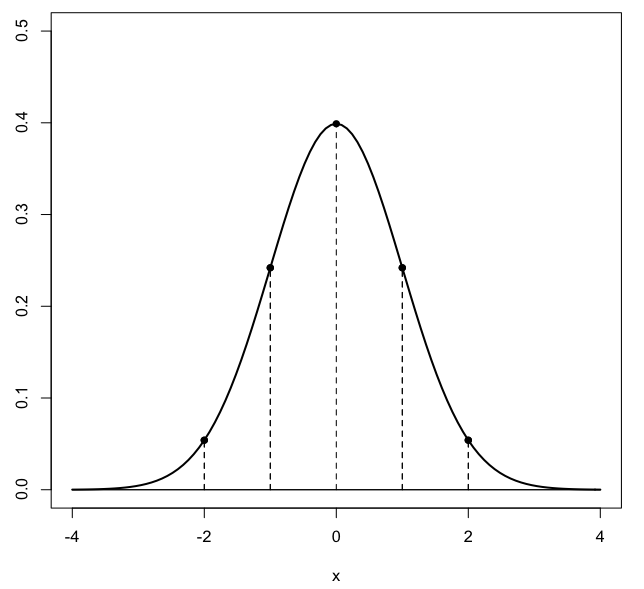
\includegraphics [scale=0.4] {gauss3.png} \end{center}

\title{Work, energy and potential}
\date{}

\begin{document}
\maketitle
\Large
To keep things simple, in this chapter we will use only one dimension.  The beauty of orthogonal directions (or \emph{basis vectors} for space) is independence:  the net force or displacement or whatever we care about is the sum of what happens in $x$, plus what happens in $y$, and the same for $z$.

The second nice feature is that when two vectors are not parallel, say the force and the distance, then we take the component which is in the same direction using the dot product:  $\mathbf{F} \cdot d \mathbf{r} = F \cos \theta \times r$.  If we adopt the convention that this has already been done implicitly, then we can just write force times distance or $Fd$.

The only thing left is to deal with the fact that in some cases the force might not be constant over distance (or time or whatever pieces we're adding up), so we set up the integral $\int F dx$ and add up for each piece the value of $F$ for the corresponding position $x_i$.

\subsection*{work-energy}

Previously, we \label{sec:Gravity}\hyperref[sec:Falling_bodies]{\textbf{derived}} this relationship for motion with acceleration $a$:
\[ v^2 - v_0^2 = 2a (x - x_0) \]

starting from the basic equation of motion
\[ x = \frac{1}{2}at^2 + v_0t + x_0 \]
and the fact that velocity is the time-derivative of position
\[ v = \frac{dx}{dt} = 2a + v_0 \]

Newton's second law says that $a = F/m$ so
\[ v^2 - v_0^2 = 2a (x - x_0) \]
\[ v^2 - v_0^2 = 2\frac{F}{m} (x - x_0) \]
Rearranging
\[ \frac{1}{2}mv^2 -  \frac{1}{2}mv_0^2 = F (x - x_0) \]

The term $\frac{1}{2} mv^2$ is called the kinetic energy.  The change in kinetic energy is equal to the force, times the distance over which it operates.
\[ K - K_0 = \Delta K = Fd \]
If the force is not constant then
\[ \Delta K = \int F \ dx \]

We make another definition:  $Fd$ is the work done by the force
\[ W = Fd = \Delta K \]

Suppose we take our marble back up to the leaning Tower of Pisa and drop it, then the work done by the force of gravity on the marble during its fall through height $h$ is $W = Fd = mgh$, which is equal to the kinetic energy acquired during the fall.  If the initial velocity is zero then
\[ \frac{1}{2} mv^2 = mgh \]
\[ v = \sqrt{2gh} \]

Work has a sign.  If the work done is in the direction that the force acts, it's positive.

\subsection*{potential energy}

If we consider the marble as it is balanced on the wall at the top of the tower (or for that matter while it is still in my pocket), we say that it has more potential energy than it does before I carry it up, or after its arrival back down at the bottom.  

The change in potential energy is exactly equal to the change in kinetic energy.

There is a funny business about the sign.  By definition:
\[ \Delta K = K - K_0 = \int_{x_0}^x F \ dx \]
Suppose the function $G$ is the integral of $F \ dx$ then

\[  \Delta K = G(x) - G(x_0) = G - G_0 \]
so
\[ K - G = K_0 - G_0 \]

We don't like those minus signs.  

The solution is to define $U = -G$, where $U$ is called the potential energy.  Then
\[ K + U = K_0 + U_0 \]

This is the law of conservation of energy:  the kinetic energy $K$ plus the potential energy $U$ is constant.

Going back to $G$ we see that 
\[ G' = \frac{d}{dx} G = F \]
so
\[ -\frac{d}{dx} U = F \]
Minus the derivative of the poential energy is equal to the force.

The vector form of this relationship is
\[ - \nabla U = \mathbf{F} \]

\subsection*{visualization}
The relationships derived above are quite easy to visualize.  In practice there can be confusion about the sign, but the basic idea is simple.  

Consider this 550 foot tall "mountain" on the island of Iwo Jima.  (It has a special importance for me.  The fact that I am here (or was) is due to something that \emph{didn't} happen there but could have,  in Feb-Mar 1945).
\begin{center} 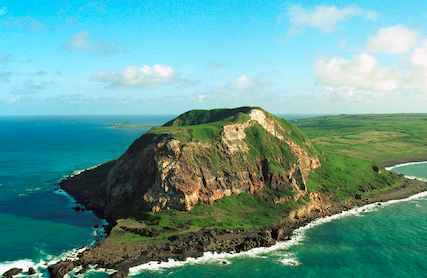
\includegraphics [scale=0.3] {suribachi1.png} \end{center}

I found a topographical map on the web 
\begin{center} 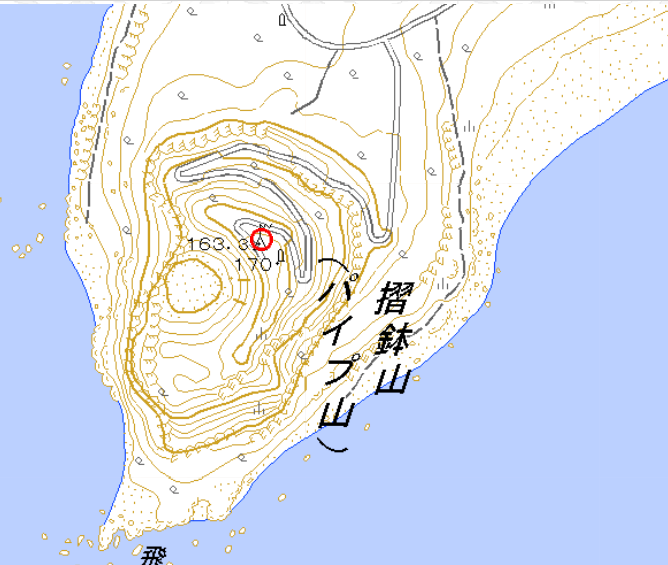
\includegraphics [scale=0.3] {suribachi2.png} \end{center}

The lines connect positions with equal height.  They connection positions of equal potential, and are what Auroux calls level curves.

The lines shown on the map are roughly circular (at least near the bottom), and the smaller the circle the greater the height.

The potential energy $U$ increases as the height increases.  The gradient of $U$, $\nabla U$ points perpendicularly to the level curves.  

$\nabla U$ points in the direction of increasing height.  If you happen to stumble and fall, however, the direction that gravity pushes you is downhill, and it will be exactly opposite to the direction in which $\nabla U$ points.  Hence $\mathbf{F} = - \nabla U$.

There are, as we said issues about sign.  For example, when work is done by a force that is increasing the potential energy, that force acts in the opposite direction from gravity or from the electric field.  Also, in electricity, we must worry about the sign of the charge that is responding to the field.

\subsection*{mass and spring}
In the mass and spring system, we find experimentally that
\[ F = - kx \]
using the definitions above we find that
\[ U = - \int F dx = \frac{1}{2} kx^2 \]
and conservation of energy says that
\[  \frac{1}{2} kx^2 +  \frac{1}{2} mv^2 = \text{const} \]

If the mass is pulled to the right for an initial displacement $A$ and then let go, at any time afterward (idealizing with no friction)
\[ \frac{1}{2} kx^2 +  \frac{1}{2} mv^2 = \frac{1}{2} kA^2 \]
\[ \frac{k}{m}(A^2 - x^2) = v^2 \]
\[ v = \sqrt{\frac{k}{m}} \sqrt{A^2 - x^2} \]

We \hyperref[sec:Harmonic_oscillator]{\textbf{solved}} the differential equation of this system
\[ F = -kx = ma = m \ddot x \]
\[ \ddot x + \frac{k}{m} x = 0 \]
One solution is
\[ x(t) = A \cos \omega t \]
\[ \ddot x(t) = -\omega^2 x(t) = -\frac{k}{m} x(t)\]
so 
\[ \omega^2 = \frac{k}{m} \]
\[ \omega = \pm \ \frac{k}{m} \]
$\omega$ is the angular frequency (it is called that because one can view the oscillation as the projection of circular motion onto one dimension).

Going back to the equation for the velocity

\[ v = \pm \ \omega \sqrt{A^2 - x^2} \]
If we want the velocity for $x = 0$ it is just $v = \pm \ A \omega$.
It is plus or minus depending on the direction of travel.

If the time $t$ is equal to one period $t = T$, then the product $\omega T$ is equal to $2 \pi$ so $\omega = 2 \pi / T$.  The units are radians per second.  One can also write $\omega = 2 \pi f$ where $f$ is the frequency.

\subsection*{potential}

The last topic for this chapter is potential.  Potential is not the same as potential energy.  It is rather, that work done by a force, gravitational or electrical or whatever, \emph{on a unit charge or mass}.

Let's start with the force itself.  As our example, take the electric force.

The force exerted at a point on a unit test charge is called the electric field $\mathbf{E}$.  Let's agree to work in one dimension so that $\mathbf{F} = F$ and $\mathbf{E} = E$ and so on.  Then
\[ F = qE \]

Now recall from above that the work $W = Fd$, work is the product of force times distance.  

Potential is the work with the charge separated out, it is
\[ W = qEd = qV \]
\[ V = Ed \]
Potential is also called \emph{voltage} and has units of volts.

Electric field strength is defined in terms of newtons per coulomb, which now makes sense.  One volt is defined as one joule per coulomb.

Power is the time-derivative of the work
\[ P = \frac{d}{dt} W = \frac{d}{dt} \ qEd \]
So, for a constant electric field, since current $i = dq/dt$
\[ P = iEd = Vi \]
and if the resistor follows Ohm's Law ($i = V/R$) then
\[ P = Vi = i^2 R \]

\subsection*{example}
A light bulb has a resistance of $R = 240 \Omega$.  If the circuit is $120 V$, then the current will be $i = V/R = 0.5 A$, one-half an amp, and the power will be
\[ P = i^2 R = 60 W \]
60 watts.

In my shop I have a tool with a $1-1/2$ hp (horsepower) motor.  $1$ hp $= 746 W$.  The current it draws is $P/V = 1119 W / 120 V = 9.3 A$.  That should be OK for a standard $15$ amp circuit.

\subsection*{ski jumper}
This problem doesn't have any calculus in it but it's still fun.

\begin{center} 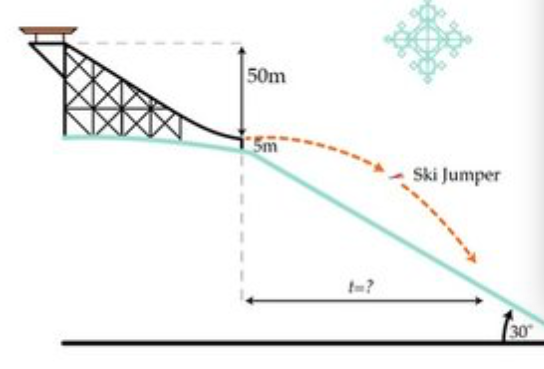
\includegraphics [scale=0.6] {ski_jumper.png} \end{center}
A ski jumper goes down a ramp of 50 meters height which is the same angle as the slope, 30 degrees.  At the very end of the ramp all velocity is converted into horizontal motion by a small lip.  We may not neglect friction:  the coefficient of kinetic friction $\mu = 0.05$.

Given some horizontal velocity $v$, the equations of motion (taking $y$ positive downward) are:
\[ x = vt \]
\[ y = \frac{1}{2} gt^2 -5 \]
(We take the origin of coordinates to be 5 m below the release point.)  Solve for the time when
\[ \frac{y}{x} = \tan \theta = \frac{1}{\sqrt{3}} \]
If we can ignore the extra 5 feet, we would have
\[ \tan \theta = \frac{g}{2v} t \]
\[ t = \frac{2v}{g \sqrt{3}} \]
\[ x = v^2 \frac{2}{g \sqrt{3}} = \frac{v^2}{g \cos \theta}  \]
If we cannot neglect it we have
\[ \tan \theta = \frac{g}{2v} t - \frac{5}{vt} \]
\[ \frac{1}{2}gt^2 - v \tan \theta \ t - 5  = 0 \]
Given $v$  we can solve for $t$ and then compute $vt$.

\subsection*{first part}
The force of gravity is $mg$, reduced by the factor of $\cos \theta$.  The force which determines friction is that pointed perpendicular into the slope, $mg \sin \theta$.  Friction opposes gravity along the ramp, giving a net force of
\[ mg \cos \theta - \mu mg \sin \theta \]
The work done is the force times the distance, the length of the ramp, which is $h \sin \theta$.  We have
\[ W = mgh(\cos \theta - \mu \sin \theta) \sin \theta \]
This is equal to the kinetic energy at take-off so
\[ \frac{1}{2} \ mv^2 = mgh(\cos \theta - \mu \sin \theta) \sin \theta \]
\[ v^2 = 2gh(\cos \theta - \mu \sin \theta) \sin \theta \]
so finally
\[ x = \frac{1}{g \cos \theta} \ 2gh(\cos \theta - \mu \sin \theta) \sin \theta \]
\[ = 2h \ (1 - \mu \tan \theta) \sin \theta \]
\[ = 100 \ (1 - \frac{0.05}{\sqrt{3}}) \frac{1}{2} = 50 - \frac{2.5}{\sqrt{3}} \]

\end{document}